\subsection{MSVC: x86}

Here is what we get in the assembly output (MSVC 2010):

\lstinputlisting{patterns/04_scanf/3_checking_retval/ex3_MSVC_x86.asm}

\index{x86!\Registers!EAX}
The \gls{caller} function (\main) needs the \gls{callee} function (\scanf) result, 
so the \gls{callee} returns it in the \EAX register.

\index{x86!\Instructions!CMP}
We check it with the help of the instruction \TT{CMP EAX, 1} (\IT{CoMPare}). In other words, we compare the value in the \EAX register with 1.

\index{x86!\Instructions!JNE}
A \JNE conditional jump follows the \CMP instruction. \JNE stands for \IT{Jump if Not Equal}.

So, if the value in the \EAX register is not equal to 1, the \ac{CPU} will pass the execution to the address mentioned in the \JNE operand, in our case \TT{\$LN2@main}.
Passing the control to this address results in the \ac{CPU} executing \printf with the argument \TT{What you entered? Huh?}.
But if everything is fine, the conditional jump is not be be taken, and another \printf call is to be executed, with two arguments: \TT{'You entered \%d...'} and the value of \TT{x}.

\index{x86!\Instructions!XOR}
\index{\CLanguageElements!return}
Since in this case the second \printf has not to be executed, there is a \JMP preceding it (unconditional jump). 
It passes the control to the point after the second \printf and just before the \TT{XOR EAX, EAX} instruction, which implements \TT{return 0}.

% FIXME internal \ref{} to x86 flags instead of wikipedia
\index{x86!\Registers!\Flags}
So, it could be said that comparing a value with another is \IT{usually} implemented by \CMP/\Jcc instruction pair, where \IT{cc} is \IT{condition code}.
\CMP compares two values and sets processor flags\footnote{x86 flags, see also: \href{http://go.yurichev.com/17120}{wikipedia}.}.
\Jcc checks those flags and decides to either pass the control to the specified address or not.

\index{x86!\Instructions!CMP}
\index{x86!\Instructions!SUB}
\index{x86!\Instructions!JNE}
\index{x86!\Registers!ZF}
\label{CMPandSUB}
This could sound paradoxical, but the \CMP instruction is in fact \SUB (subtract).
All arithmetic instructions set processor flags, not just \CMP.
If we compare 1 and 1, $1-1$ is 0 so the \ZF flag would be set (meaning that the last result was 0).
In no other circumstances \ZF can be set, except when the operands are equal.
\JNE checks only the \ZF flag and jumps only if it is not set.  \JNE is in fact a synonym for \JNZ (\IT{Jump if Not Zero}).
Assembler translates both \JNE and \JNZ instructions into the same opcode.
So, the \CMP instruction can be replaced with a \SUB instruction and almost everything will be fine, with the difference that \SUB alters the value of the first operand.
\CMP is \IT{SUB without saving the result, but affecting flags}.

\ifx\LITE\undefined
\subsection{MSVC: x86: IDA}

\index{IDA}
It is time to run \IDA and try to do something in it.
By the way, for beginners it is good idea to use \TT{/MD} option in MSVC, which means that all these
standard functions are not be linked with the executable file, 
but are to be imported from the \TT{MSVCR*.DLL} file instead.
Thus it will be easier to see which standard function are used and where.

While analysing code in \IDA, it is very helpful to leave notes for oneself (and others).
In instance, analysing this example, 
we see that \TT{JNZ} is to be triggered in case of an error.
So it is possible to move the cursor to the label, press \q{n} and rename it to \q{error}.
Create another label---into \q{exit}.
Here is my result:

\lstinputlisting{patterns/04_scanf/3_checking_retval/ex3.lst}

Now it is slightly easier to understand the code.
However, it is not a good idea to comment on every instruction.

% FIXME draw button?
You could also hide(collapse) parts of a function in \IDA.
To do that mark the block, then press \q{--} on the numerical pad and enter the text to be displayed instead.

Let's hide two blocks and give them names:

\lstinputlisting{patterns/04_scanf/3_checking_retval/ex3_2.lst}

% FIXME draw button?
To expand previously collapsed parts of the code, use \q{+} on the numerical pad.

\clearpage
By pressing \q{space}, we can see how \IDA represents a function as a graph:

\begin{figure}[H]
\centering
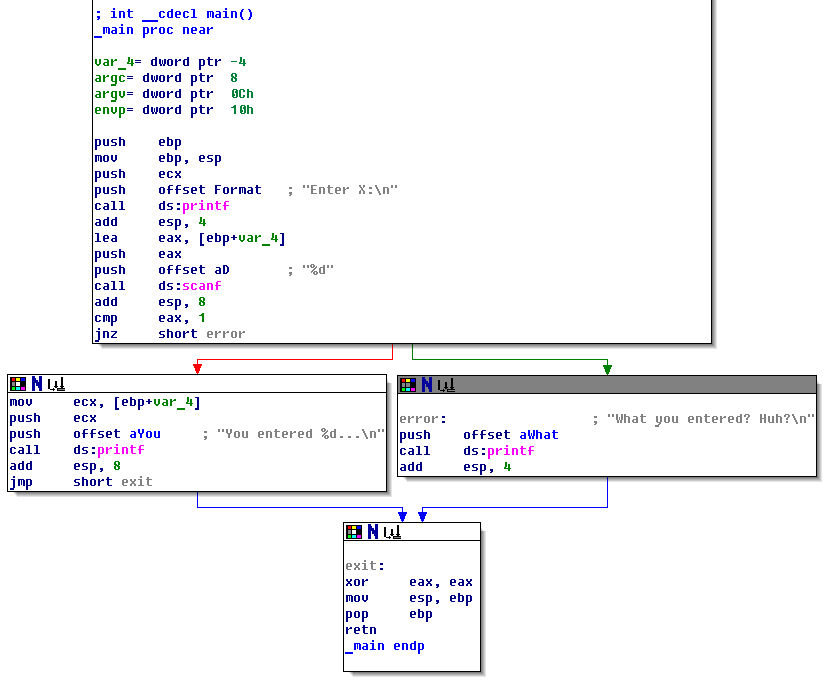
\includegraphics[scale=\FigScale]{patterns/04_scanf/3_checking_retval/IDA.png}
\caption{Graph mode in IDA}
\label{fig:ex3_IDA_1}
\end{figure}

There are two arrows after each conditional jump: green and red.
The green arrow points to the block which executes if the jump is triggered, and red if otherwise.

\clearpage
It is possible to fold nodes in this mode and give them names as well (\q{group nodes}).
Let's do it for 3 blocks:

\begin{figure}[H]
\centering
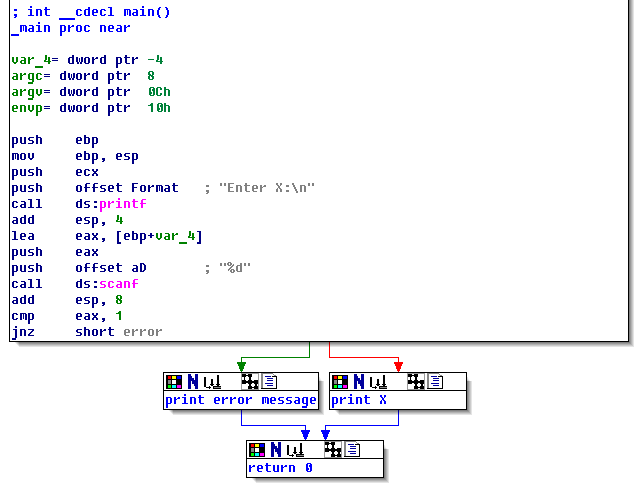
\includegraphics[scale=\FigScale]{patterns/04_scanf/3_checking_retval/IDA2.png}
\caption{Graph mode in IDA with 3 nodes folded}
\label{fig:ex3_IDA_2}
\end{figure}

That is very useful.
It could be said that a very important part of the reverse engineers' job (and any other researcher as well) is to reduce the amount of information they deal with.
\fi

\ifdefined\IncludeOlly
\clearpage
\subsection{MSVC: x86 + \olly}

\RU{Попробуем в \olly немного хакнуть программу и сделать вид, что \scanf срабатывает всегда без ошибок.}
\EN{Let's try to hack our program in \olly, forcing it to think \scanf always works without error.}

\RU{Когда в \scanf передается адрес локальной переменной, изначально в этой переменной
находится некий мусор. В данном случае это}\EN{When an address of a local variable is passed into \scanf,
the variable initially contains some random garbage, in this case} \TT{0x6E494714}:

\begin{figure}[H]
\centering
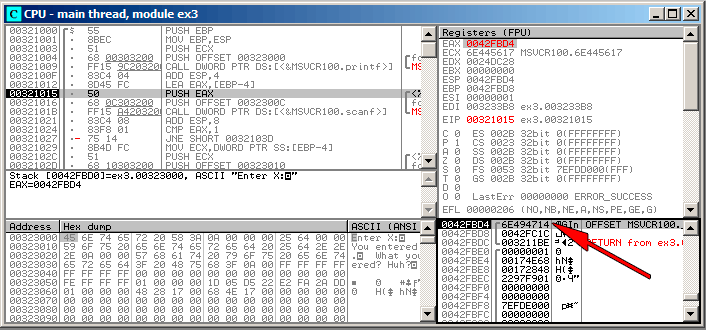
\includegraphics[scale=\FigScale]{patterns/04_scanf/3_checking_retval/olly_1.png}
\caption{\olly: \RU{передача адреса переменной в}\EN{passing variable address into} \scanf}
\label{fig:scanf_ex3_olly_1}
\end{figure}

\clearpage
\RU{Когда}\EN{While} \scanf \RU{запускается, я ввожу в консоли что-то непохожее на число, например}
\EN{executes, in the console I enter something that is definitely not a number, like} ``asdasd''.
\scanf \RU{заканчивается с 0 в}\EN{finishes with 0 in} \EAX, \RU{что означает, что произошла ошибка}%
\EN{which indicates that an error has occurred}:

\begin{figure}[H]
\centering
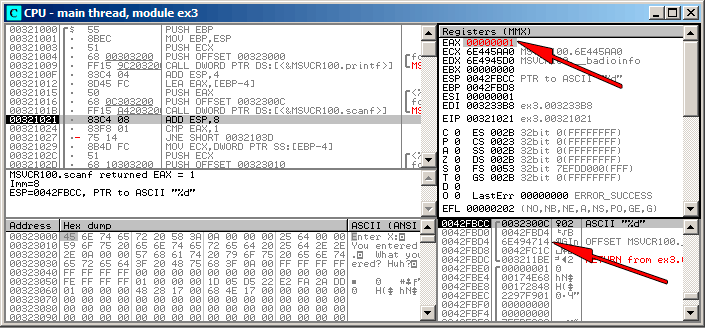
\includegraphics[scale=\FigScale]{patterns/04_scanf/3_checking_retval/olly_2.png}
\caption{\olly: \scanf \RU{закончился с ошибкой}\EN{returning error}}
\label{fig:scanf_ex3_olly_2}
\end{figure}

\RU{Вместе с этим мы можем посмотреть на локальную переменную в стеке~--- она не изменилась.}
\EN{We can also check the local variable in the stack and note that it has not changed.}
\RU{Действительно, ведь что туда записала бы функция \scanf}\EN{Indeed, what would \scanf write there}?
\RU{Она не делала ничего кроме возвращения нуля}\EN{It simply did nothing except returning zero}.

\RU{Попробуем ещё немного ``хакнуть'' нашу программу}\EN{Let's try to ``hack'' our program}.
\RU{Щелкнем правой кнопкой на}\EN{Right-click on} \EAX, \RU{там, в числе опций, будет также}
\EN{Among the options there is} ``Set to 1''.
\RU{Это нам и нужно}\EN{This is what we need}.

\RU{В \EAX теперь 1, последующая проверка пройдет как надо, и \printf выведет значение переменной
из стека.}
\EN{We now have 1 in \EAX, so the following check is to be executed as intended, 
and \printf will print the value of the variable in the stack.}

\RU{Запускаем (F9) и видим в консоли следующее:}
\EN{When we run the program (F9) we can see the following in the console window:}

\begin{figure}[H]
\centering
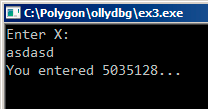
\includegraphics[scale=\FigScale]{patterns/04_scanf/3_checking_retval/olly_3.png}
\caption{\RU{консоль}\EN{console window}}
\end{figure}

\RU{Действительно}\EN{Indeed}, $1850296084$ \RU{это десятичное представление числа в стеке}
\EN{is a decimal representation of the number in the stack} (\TT{0x6E494714})!

\fi

\clearpage
\subsection{MSVC: x86 + Hiew}
\index{Hiew}

This can also be used as a simple example of executable file patching.
We may try to patch the executable so the program would always print the input, no matter what we enter.

Assuming that the executable is compiled against external \TT{MSVCR*.DLL} (i.e., with \TT{/MD} option)
\footnote{that's what also called \q{dynamic linking}}, 
we see the \main function at the beginning of the \TT{.text} section.
Let's open the executable in Hiew and find the beginning of the \TT{.text} section (Enter, F8, F6, Enter, Enter).

We can see this:

\begin{figure}[H]
\centering
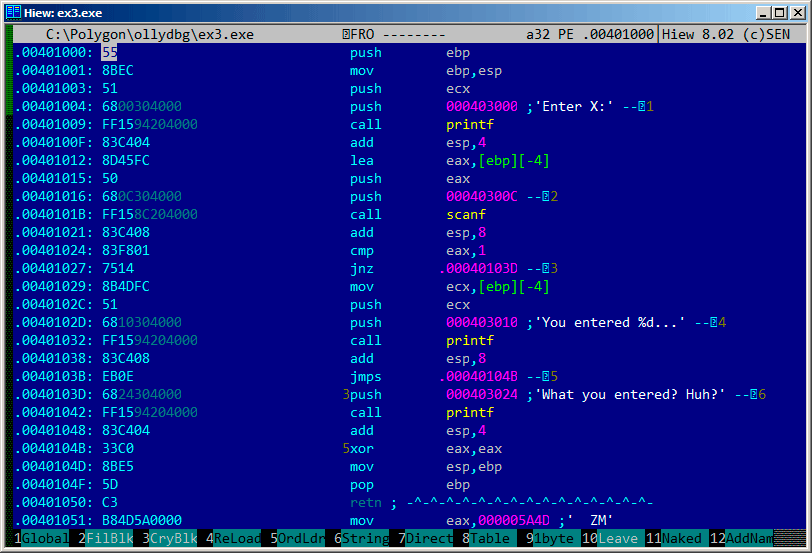
\includegraphics[scale=\FigScale]{patterns/04_scanf/3_checking_retval/hiew_1.png}
\caption{Hiew: \main function}
\label{fig:scanf_ex3_hiew_1}
\end{figure}

Hiew finds \ac{ASCIIZ} strings and displays them, as it does with the imported functions' names.

\clearpage
Move the cursor to address \TT{.00401027} (where the \TT{JNZ} instruction, we have to bypass, is located), press F3, and then type \q{9090} (meaning two \ac{NOP}s):

\begin{figure}[H]
\centering
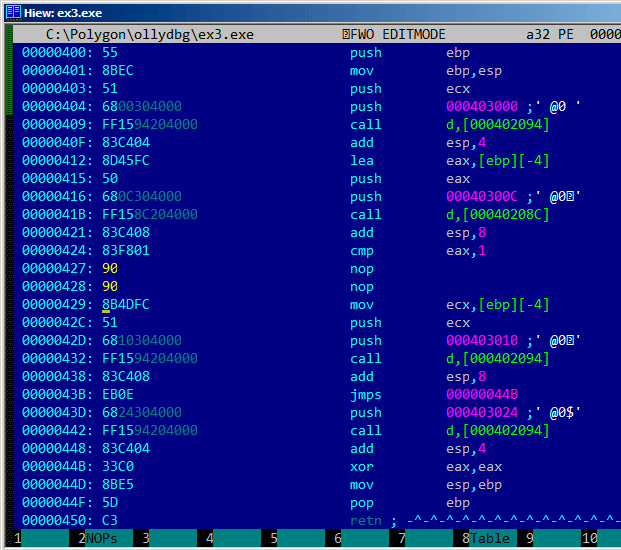
\includegraphics[scale=\FigScale]{patterns/04_scanf/3_checking_retval/hiew_2.png}
\caption{Hiew: replacing \TT{JNZ} with two \ac{NOP}s}
\label{fig:scanf_ex3_hiew_2}
\end{figure}

Then press F9 (update). Now the executable is saved to the disk. It will behave as we wanted.

Two \ac{NOP}s are probably not the most \ae{}sthetic approach.
Another way to patch this instruction is to write just 0 to the second opcode byte (\gls{jump offset}), 
so that \TT{JNZ} will always jump to the next instruction.

We could also do the opposite: replace first byte with \TT{EB} while not touching the second byte (\gls{jump offset}).
We would get an unconditional jump that is always triggered.
In this case the error message would be printed every time, no matter the input.

